\documentclass[tikz,border=5pt]{standalone}
\begin{document}
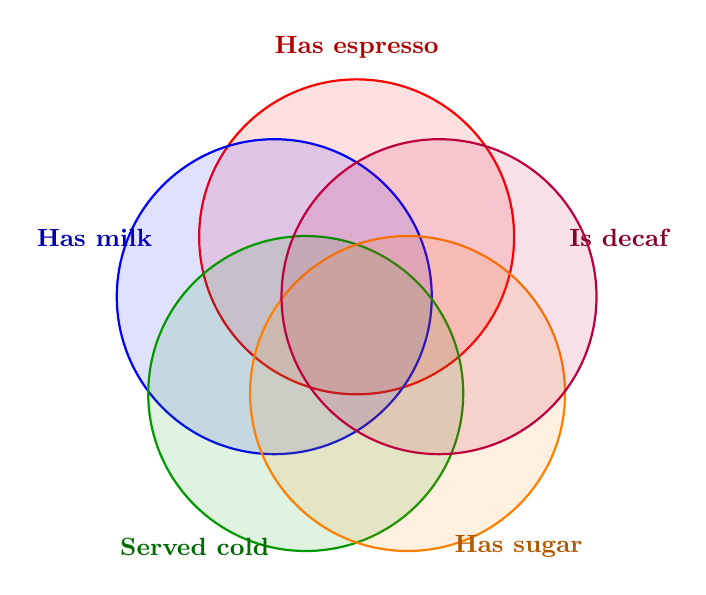
\begin{tikzpicture}
\foreach \i/\n/\c in {0/Has espresso/red,1/Has milk/blue,2/Served cold/green!60!black,3/Has sugar/orange,4/Is decaf/purple}{
 \draw[\c,thick,fill=\c,fill opacity=0.12] ({90+72*\i}:1.1) circle (2);
 \node[\c!70!black,font=\small\bfseries,align=center] at ({90+72*\i}:3.5) {\n};
}
\end{tikzpicture}
\end{document}
